\documentclass{beamer}
\usepackage[utf8]{inputenc}
\usepackage[T1]{fontenc}
\usepackage{graphicx}
\usepackage{xcolor}
\usepackage{listings}
\usepackage{tikz}
\usepackage{amsmath}
\usepackage{hyperref}
\usepackage{bookmark}

% Theme - Import oppstar theme from beamer-template directory
% Add beamer-template directory to LaTeX search path
\makeatletter
\def\input@path{{./beamer-template/}}
\makeatother

% Now load the theme components
\usepackage{./beamer-template/beamercolorthemeoppstar}
\usepackage{./beamer-template/beamerfontthemeoppstar}
\usepackage{./beamer-template/beamerinnerthemeoppstar}
\usepackage{./beamer-template/beamerouterthemeoppstar}
\usepackage{./beamer-template/beamerthemeoppstar}

% Colors
\definecolor{codeblue}{RGB}{0,102,204}
\definecolor{codegray}{RGB}{128,128,128}
\definecolor{codegreen}{RGB}{0,128,0}
\definecolor{backcolour}{RGB}{245,245,245}

% Code listing style
\lstdefinestyle{cstyle}{
    backgroundcolor=\color{backcolour},
    commentstyle=\color{codegreen},
    keywordstyle=\color{codeblue},
    numberstyle=\tiny\color{codegray},
    stringstyle=\color{red},
    basicstyle=\ttfamily\footnotesize,
    breakatwhitespace=false,
    breaklines=true,
    keepspaces=true,
    numbers=left,
    numbersep=5pt,
    showspaces=false,
    showstringspaces=false,
    showtabs=false,
    tabsize=2,
    frame=single
}

\lstset{style=cstyle}

% Title page info
\title{Day 6: Capstone Project and Course Synthesis}
\subtitle{C Programming for Post-Silicon Validation Engineers}
\author{Course Instructor}
\date{6-Day Intensive Bootcamp}
\institute{Post-Silicon Validation Training Program}

\begin{document}

\frame{\titlepage}

\begin{frame}
\frametitle{Welcome to Day 6!}
\begin{center}
\Large The Grand Finale: Your Validation Masterpiece
\end{center}

\begin{itemize}
    \item \textbf{Journey So Far:} From zero to embedded validation expert
    \item \textbf{Today's Mission:} Integrate everything into a capstone project
    \item \textbf{Validation Focus:} Complete end-to-end validation system
    \item \textbf{Team Collaboration:} Work together on complex projects
    \item \textbf{Outcome:} Professional portfolio and presentation!
\end{itemize}

\vspace{0.5cm}
\begin{center}
\textit{``The expert in anything was once a beginner''} - Helen Hayes
\end{center}
\end{frame}

\begin{frame}
\frametitle{Your Amazing Journey}
\begin{center}
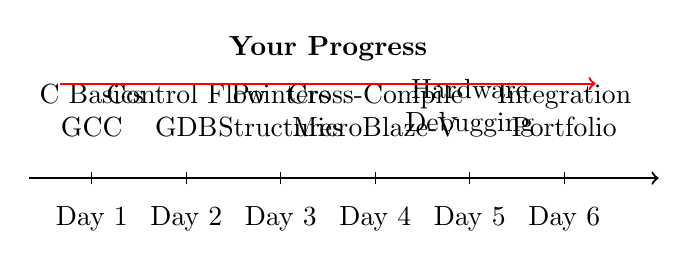
\begin{tikzpicture}[scale=0.8]
% Timeline
\draw[thick, ->] (0,0) -- (10,0);

% Day markers
\foreach \x/\day in {1/Day 1, 2.5/Day 2, 4/Day 3, 5.5/Day 4, 7/Day 5, 8.5/Day 6} {
    \draw (\x,-0.1) -- (\x,0.1);
    \node[below] at (\x,-0.3) {\day};
}

% Skills acquired
\node[above, align=center] at (1,0.5) {C Basics\\GCC};
\node[above, align=center] at (2.5,0.5) {Control Flow\\GDB};
\node[above, align=center] at (4,0.5) {Pointers\\Structures};
 \node[above, align=center] at (5.5,0.5) {Cross-Compile\\MicroBlaze-V};
\node[above, align=center] at (7,0.5) {Hardware\\Debugging};
\node[above, align=center] at (8.5,0.5) {Integration\\Portfolio};

% Progress arrow
\draw[thick, red, ->] (0.5,1.5) -- (9,1.5);
\node[above] at (4.75,1.7) {\textbf{Your Progress}};
\end{tikzpicture}
\end{center}

\vspace{0.5cm}
\textbf{What you've mastered:}
\begin{itemize}
    \item C programming fundamentals and advanced concepts
    \item Professional development tools and workflows
    \item Embedded systems programming for ARM Cortex-M0+
    \item Hardware validation techniques and best practices
    \item AI-assisted development and critical evaluation
\end{itemize}
\end{frame}

\begin{frame}
\frametitle{Today's Learning Objectives}
By the end of Day 6, you will:

\begin{enumerate}
    \item Integrate all course concepts into a comprehensive project
    \item Demonstrate professional project management skills
    \item Create and deliver technical presentations
    \item Build a portfolio-ready GitHub repository
    \item Plan your continued learning journey
    \item Network with peers and establish professional connections
\end{enumerate}

\vspace{0.5cm}
\begin{alertblock}{Capstone Day}
Today you prove you're ready for post-silicon validation roles!
\end{alertblock}
\end{frame}

\begin{frame}
\frametitle{Capstone Project Overview}
\textbf{Project Goal:} Design and implement a comprehensive validation system that demonstrates all course concepts.

\vspace{0.5cm}
\textbf{Team Structure:}
\begin{itemize}
    \item Teams of 2-3 participants
    \item Diverse skill combinations encouraged
    \item Collaborative development using GitHub
    \item Peer code reviews and knowledge sharing
\end{itemize}

\vspace{0.5cm}
\textbf{Time Allocation:}
\begin{itemize}
    \item \textbf{Planning \& Design:} 1 hour
    \item \textbf{Implementation:} 4 hours
    \item \textbf{Testing \& Documentation:} 1 hour
    \item \textbf{Presentations:} 1 hour
\end{itemize}
\end{frame}

\begin{frame}
\frametitle{Project Requirements}
\textbf{Core Requirements (Must Have):}
\begin{enumerate}
    \item Multi-peripheral validation (GPIO, ADC, timers)
    \item Modular code architecture with headers
    \item Cross-compilation for MicroBlaze-V
    \item Hardware-in-the-loop testing
    \item Error handling and recovery
    \item Professional documentation
\end{enumerate}

\vspace{0.5cm}
\textbf{Advanced Features (Choose 2+):}
\begin{itemize}
    \item Fault injection and recovery testing
    \item Statistical analysis of test results
    \item Real-time performance monitoring
    \item Automated test report generation
    \item AI-assisted code optimization
    \item Custom validation protocols
\end{itemize}
\end{frame}

\begin{frame}
\frametitle{Project Ideas and Inspiration}
\textbf{Suggested Project Themes:}

\begin{enumerate}
    \item \textbf{Multi-Chip Validation Suite:} Test multiple MicroBlaze-V boards simultaneously
    \item \textbf{Environmental Stress Tester:} Validate under temperature/voltage variations
    \item \textbf{Communication Protocol Validator:} Test UART/SPI/I2C interfaces
    \item \textbf{Power Management Tester:} Validate sleep modes and power consumption
    \item \textbf{Signal Integrity Analyzer:} Test signal quality and timing
    \item \textbf{Automated Regression Tester:} Continuous validation framework
\end{enumerate}

\vspace{0.5cm}
\textbf{Innovation Encouraged:}
\begin{itemize}
    \item Combine multiple themes
    \item Add unique validation scenarios
    \item Implement creative user interfaces
    \item Develop novel testing methodologies
\end{itemize}
\end{frame}

\begin{frame}[fragile]
\frametitle{Project Architecture Template}
\begin{lstlisting}[basicstyle=\tiny\ttfamily]
Project structure example:
validation_suite/
|-- src/
|   |-- main.c                 // Main application
|   |-- validation_core.c      // Core validation logic
|   |-- hardware_abstraction.c // HAL layer
|   |-- test_suites.c         // Individual test implementations
|   |-- fault_injection.c     // Fault testing
|   |-- reporting.c           // Results and statistics
|   +-- ai_optimization.c     // AI-assisted features
|-- include/
|   |-- validation_core.h
|   |-- hardware_abstraction.h
|   |-- test_suites.h
|   +-- common_types.h
|-- tests/
|   |-- unit_tests.c          // Unit test suite
|   +-- integration_tests.c   // Integration tests
|-- docs/
|   |-- README.md             // Project documentation
|   |-- API_reference.md      // Function documentation
|   +-- user_guide.md         // Usage instructions
|-- CMakeLists.txt            // Build configuration
+-- .github/
    +-- workflows/
        +-- ci.yml            // Continuous integration
\end{lstlisting}
\end{frame}

\begin{frame}[fragile]
\frametitle{Sample Capstone Code Structure}
\begin{lstlisting}[language=C, basicstyle=\tiny]
// validation_core.h - Main interface
#ifndef VALIDATION_CORE_H
#define VALIDATION_CORE_H

#include <stdint.h>
#include <stdbool.h>

typedef struct {
    char test_name[64];
    bool passed;
    uint32_t execution_time_us;
    char error_message[128];
} test_result_t;

typedef struct {
    uint32_t total_tests;
    uint32_t passed_tests;
    uint32_t failed_tests;
    float success_rate;
    uint32_t total_execution_time_us;
} validation_summary_t;

// Core validation functions
int initialize_validation_system(void);
int run_comprehensive_validation(validation_summary_t *summary);
int run_specific_test_suite(const char *suite_name, test_result_t results[]);
void generate_validation_report(const validation_summary_t *summary);
void cleanup_validation_system(void);

// Test suite functions
int run_gpio_validation_suite(test_result_t results[]);
int run_adc_validation_suite(test_result_t results[]);
int run_timing_validation_suite(test_result_t results[]);
int run_fault_injection_suite(test_result_t results[]);

#endif // VALIDATION_CORE_H
\end{lstlisting}
\end{frame}

\begin{frame}
\frametitle{Team Formation and Roles}
\textbf{Team Formation Strategy:}
\begin{itemize}
    \item Mix of different skill levels and backgrounds
    \item Complementary strengths (hardware focus, software focus, etc.)
    \item Good communication and collaboration potential
    \item Shared interest in project theme
\end{itemize}

\vspace{0.5cm}
\textbf{Suggested Roles:}
\begin{itemize}
    \item \textbf{Project Lead:} Overall coordination and integration
    \item \textbf{Hardware Specialist:} MicroBlaze-V programming and debugging
    \item \textbf{Software Architect:} Code structure and optimization
    \item \textbf{Quality Engineer:} Testing and validation
    \item \textbf{Documentation Lead:} README, comments, and presentation
\end{itemize}

\vspace{0.5cm}
\textbf{Note:} In 2-3 person teams, members wear multiple hats!
\end{frame}

\begin{frame}
\frametitle{Project Planning Session}
\textbf{Planning Checklist (30 minutes):}

\begin{enumerate}
    \item \textbf{Project Selection:} Choose theme and scope
    \item \textbf{Requirements Definition:} Core and advanced features
    \item \textbf{Architecture Design:} Module breakdown and interfaces
    \item \textbf{Task Assignment:} Who does what and when
    \item \textbf{GitHub Setup:} Repository creation and branch strategy
    \item \textbf{Milestone Planning:} Hourly checkpoints and deliverables
\end{enumerate}

\vspace{0.5cm}
\textbf{Planning Tools:}
\begin{itemize}
    \item GitHub Projects for task tracking
    \item Shared Google Doc for design notes
    \item Whiteboard for architecture diagrams
    \item Timer for milestone management
\end{itemize}
\end{frame}

\begin{frame}
\frametitle{Development Best Practices}
\textbf{Collaborative Development:}
\begin{itemize}
    \item \textbf{Frequent commits:} Small, focused changes
    \item \textbf{Descriptive messages:} Clear commit descriptions
    \item \textbf{Branch strategy:} Feature branches with pull requests
    \item \textbf{Code reviews:} Peer review before merging
    \item \textbf{Continuous integration:} Automated testing
\end{itemize}

\vspace{0.5cm}
\textbf{Quality Assurance:}
\begin{itemize}
    \item \textbf{Unit testing:} Test individual functions
    \item \textbf{Integration testing:} Test module interactions
    \item \textbf{Hardware testing:} Validate on actual MicroBlaze-V
    \item \textbf{Performance testing:} Measure execution times
    \item \textbf{Documentation:} Keep README updated
\end{itemize}
\end{frame}

\begin{frame}
\frametitle{AI Integration Guidelines}
\textbf{Responsible AI Usage:}
\begin{itemize}
    \item \textbf{Code Generation:} Use AI for boilerplate and complex algorithms
    \item \textbf{Optimization:} Ask AI for performance improvement suggestions
    \item \textbf{Debugging:} Get AI help with error analysis
    \item \textbf{Documentation:} AI-assisted comment and README generation
    \item \textbf{Testing:} AI-generated test cases and edge conditions
\end{itemize}

\vspace{0.5cm}
\textbf{Documentation Requirements:}
\begin{itemize}
    \item Note all AI assistance in commit messages
    \item Include AI evaluation section in README
    \item Explain why AI suggestions were accepted/rejected
    \item Demonstrate understanding of AI-generated code
    \item Show improvements made to AI suggestions
\end{itemize}
\end{frame}

\begin{frame}
\frametitle{Presentation Guidelines}
\textbf{Presentation Structure (7-10 minutes):}
\begin{enumerate}
    \item \textbf{Introduction (1 min):} Team and project overview
    \item \textbf{Problem Statement (1 min):} What validation challenge you solved
    \item \textbf{Solution Architecture (2 min):} High-level design and approach
    \item \textbf{Technical Implementation (3 min):} Key code and algorithms
    \item \textbf{Demonstration (2 min):} Live demo on MicroBlaze-V hardware
    \item \textbf{Results \& Lessons (1 min):} What worked, what you learned
\end{enumerate}

\vspace{0.5cm}
\textbf{Presentation Tips:}
\begin{itemize}
    \item Focus on validation engineering relevance
    \item Show actual code and hardware
    \item Highlight innovative features
    \item Discuss challenges and solutions
    \item Demonstrate professional communication
\end{itemize}
\end{frame}

\begin{frame}
\frametitle{Evaluation Criteria}
\textbf{Technical Implementation (40\%):}
\begin{itemize}
    \item Code quality and organization
    \item Proper use of course concepts
    \item Hardware integration effectiveness
    \item Error handling and robustness
\end{itemize}

\textbf{Innovation \& Problem Solving (25\%):}
\begin{itemize}
    \item Creative approach to validation challenges
    \item Advanced feature implementation
    \item Novel use of MicroBlaze-V capabilities
    \item AI integration effectiveness
\end{itemize}

\textbf{Collaboration \& Process (20\%):}
\begin{itemize}
    \item GitHub workflow and commit quality
    \item Team collaboration effectiveness
    \item Code review participation
    \item Project management skills
\end{itemize}

\textbf{Communication \& Documentation (15\%):}
\begin{itemize}
    \item Presentation quality and clarity
    \item Documentation completeness
    \item Professional communication
    \item Technical explanation accuracy
\end{itemize}
\end{frame}

\begin{frame}
\frametitle{Portfolio Development}
\textbf{Your GitHub Portfolio Should Include:}
\begin{itemize}
    \item \textbf{Professional README:} Clear project description and setup
    \item \textbf{Code Quality:} Well-commented, organized source code
    \item \textbf{Documentation:} API reference and user guides
    \item \textbf{Demonstration:} Videos or GIFs of hardware in action
    \item \textbf{Technical Writing:} Design decisions and trade-offs
    \item \textbf{Professional Profile:} Updated GitHub profile and bio
\end{itemize}

\vspace{0.5cm}
\textbf{Career Integration:}
\begin{itemize}
    \item Link to LinkedIn profile
    \item Highlight validation engineering skills
    \item Showcase embedded systems experience
    \item Demonstrate collaborative development
    \item Show continuous learning mindset
\end{itemize}
\end{frame}

\begin{frame}
\frametitle{Milestone Checkpoints}
\textbf{Hourly Progress Checks:}

\begin{itemize}
    \item \textbf{Hour 1:} Planning complete, GitHub setup, initial code structure
    \item \textbf{Hour 2:} Core validation functions implemented and tested
    \item \textbf{Hour 3:} Hardware integration working, basic features complete
    \item \textbf{Hour 4:} Advanced features implemented, optimization complete
    \item \textbf{Hour 5:} Testing complete, documentation finalized
    \item \textbf{Hour 6:} Presentation prepared, final demo ready
\end{itemize}

\vspace{0.5cm}
\textbf{Checkpoint Activities:}
\begin{itemize}
    \item Quick team standup (5 minutes)
    \item Progress demonstration to instructors
    \item Peer team check-ins and help
    \item Adjustment of goals if needed
    \item Celebration of achievements!
\end{itemize}
\end{frame}

\begin{frame}
\frametitle{Troubleshooting and Support}
\textbf{Common Challenges and Solutions:}
\begin{itemize}
    \item \textbf{Hardware Issues:} Backup MicroBlaze-V boards available
    \item \textbf{Compilation Problems:} TAs for build system help
    \item \textbf{Git Conflicts:} Pair programming and merge assistance
    \item \textbf{Time Management:} Scope adjustment guidance
    \item \textbf{Team Dynamics:} Instructor mediation if needed
\end{itemize}

\vspace{0.5cm}
\textbf{Support Resources:}
\begin{itemize}
    \item Instructor and TA availability throughout the day
    \item Peer teams for cross-pollination of ideas
    \item Course materials and examples for reference
    \item AI tools for coding assistance
    \item Emergency backup plans for critical issues
\end{itemize}
\end{frame}

\begin{frame}
\frametitle{Beyond the Course: Your Next Steps}
\textbf{Immediate Next Steps (Week 1-2):}
\begin{itemize}
    \item Complete post-course project enhancements
    \item Update LinkedIn with new skills and projects
    \item Connect with classmates and instructors
    \item Apply learnings to current work projects
    \item Start exploring advanced embedded topics
\end{itemize}

\vspace{0.5cm}
\textbf{Medium-term Goals (Month 1-3):}
\begin{itemize}
    \item Complete extended homework assignments
    \item Contribute to open-source embedded projects
    \item Attend embedded systems meetups and conferences
    \item Pursue advanced certifications
    \item Build additional portfolio projects
\end{itemize}

\vspace{0.5cm}
\textbf{Long-term Career Development:}
\begin{itemize}
    \item Transition to post-silicon validation roles
    \item Become a mentor for future course participants
    \item Develop expertise in specialized validation areas
    \item Lead validation teams and projects
\end{itemize}
\end{frame}

\begin{frame}
\frametitle{Course Reflection and Feedback}
\textbf{Reflection Questions:}
\begin{itemize}
    \item What was your biggest learning breakthrough?
    \item Which concepts do you want to explore further?
    \item How will you apply these skills in your career?
    \item What would you tell someone considering this course?
    \item What additional topics would be valuable?
\end{itemize}

\vspace{0.5cm}
\textbf{Feedback Opportunities:}
\begin{itemize}
    \item Course evaluation survey (anonymous)
    \item One-on-one feedback sessions with instructors
    \item Peer feedback on collaboration and learning
    \item Suggestions for course improvements
    \item Testimonials for future marketing
\end{itemize}
\end{frame}

\begin{frame}
\frametitle{Alumni Network and Community}
\textbf{Staying Connected:}
\begin{itemize}
    \item Course alumni Slack workspace
    \item Monthly virtual meetups and tech talks
    \item Shared GitHub organization for projects
    \item Mentorship program (alumni helping new students)
    \item Job referral network and career support
\end{itemize}

\vspace{0.5cm}
\textbf{Giving Back:}
\begin{itemize}
    \item Volunteer as TA for future courses
    \item Share your success stories and projects
    \item Provide feedback on course improvements
    \item Mentor new engineers in your organization
    \item Contribute to course materials and examples
\end{itemize}
\end{frame}

\begin{frame}
\frametitle{Final Thoughts and Congratulations}
\begin{center}
\Large You Did It!
\end{center}

\textbf{What you've accomplished in 6 days:}
\begin{itemize}
    \item Mastered C programming from zero to advanced
    \item Learned professional embedded development workflows
    \item Built real hardware validation systems
    \item Developed collaborative software engineering skills
    \item Created a professional portfolio of projects
    \item Joined a community of validation engineers
\end{itemize}

\vspace{0.5cm}
\begin{center}
\textbf{You are now ready for post-silicon validation roles!}
\end{center}

\vspace{0.5cm}
\begin{center}
\textit{``The journey of a thousand miles begins with a single step''} - Lao Tzu\\
\textit{You've taken many steps this week!}
\end{center}
\end{frame}

\begin{frame}
\frametitle{Let's Build Something Amazing!}
\begin{center}
\Large Time for Your Capstone Project
\end{center}

\textbf{Remember:}
\begin{itemize}
    \item Focus on validation engineering relevance
    \item Collaborate effectively with your team
    \item Use all the skills you've learned
    \item Don't be afraid to be creative and innovative
    \item Ask for help when you need it
    \item Have fun and be proud of your work!
\end{itemize}

\vspace{1cm}
\begin{center}
\textbf{Go forth and validate!}
\end{center}
\end{frame}

\end{document}
